\section{Chapter 2}
\subsection{Exercises}
\begin{sol}{Exercise 2.1}
\begin{proof}
Since $a$ is positive and $x$ is also positive, the product $ax$ must be positive. 
\end{proof}

While we could go more in depth with field axioms or abstract algebra, such a short proof will do for our purposes. This is just intended as an exercise to get your brain thinking in terms of proofs and logic.
\end{sol}

\begin{sol}{Exercise 2.2}
The original statement and the negation cannot be both simultaneously true. Since, for the original statement says that if $P$ is true than $Q$ is true, while the negation says that even though $P$ is true, $Q$ is not true. This forms a logical contradiction: one statement says $Q$ is true while the other says $Q$ is false. $Q$ cannot be true and false at the same time in our standard system of logic.

However, the original statement and its converse can be true simultaneously! This is actually a very important case, in which $P \implies Q$ and $Q \implies P$. There is no such logical contradiction here. 
\end{sol}


\begin{sol}{Exercise 2.3}
What did you come up with? Here's another I came up with: the set of exercises of chapter 2 is a set! Same with chapter 1, 3, 4, or 5. The set of problems and exercises across all chapters is also a set. The set of all problems in chapter 1 which are starred is a singleton set. However, make sure the sets you come up with do not have repeats; sets in which we do consider repeats are called multisets, and we don't use them very often in this book. 
\end{sol}

\begin{sol}{Exercise 2.4}
The answer is within the subsequent text. 
\end{sol}


\begin{sol}{Exercise 2.5}
The correct answer is very difficult to stumble across. However, roughly speaking, the set of natural numbers, integers, and rational numbers are countably infinite. While the set of real numbers and complex numbers (defined on real numbers, as is assumed the case) are uncountably infinite. The specific cardinalities are much harder to find. I discuss the answer in the following text.
\end{sol}

\begin{sol}{Exercise 2.6}
We can use simple logic, reasoning with the definitions of these binary operations, to obtain the magnitudes
\[
|A \times B| = xy
\]
and
\[
|A \cup B| = x + y
\]
assuming $A \cap B = \emptyset$.
\end{sol}




\subsection{Problems}

\begin{sol}{Problem 2.1}
$|A \cup B| = |A| + |B| - |A \cap B|$

\begin{proof}
Consider the following Venn diagram.

\begin{center}
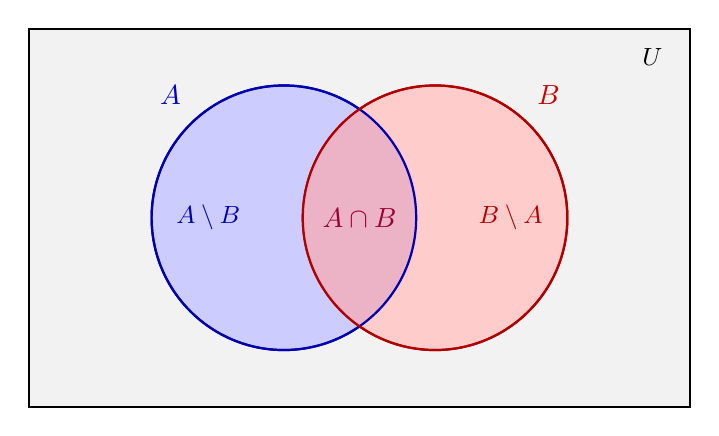
\begin{tikzpicture}[scale=1.2]

  % Universe box
  \fill[gray!10] (-3.5, -2) rectangle (3.5, 2);
  \draw[thick] (-3.5, -2) rectangle (3.5, 2);
  \node[font=\small] at (3.1, 1.7) {$U$};

  % A circle
  \fill[blue!20] (-0.8, 0) circle (1.4cm);
  \draw[thick, blue!70!black] (-0.8, 0) circle (1.4cm);

  % B circle
  \fill[red!20] (0.8, 0) circle (1.4cm);
  \draw[thick, red!70!black] (0.8, 0) circle (1.4cm);

  % Intersection fill
  \begin{scope}
    \clip (-0.8, 0) circle (1.4cm);
    \fill[purple!30] (0.8, 0) circle (1.4cm);
  \end{scope}

  % Redraw outlines on top
  \draw[thick, blue!70!black] (-0.8, 0) circle (1.4cm);
  \draw[thick, red!70!black] (0.8, 0) circle (1.4cm);

  % Labels
  \node[blue!80!black,   font=\bfseries] at (-2.0,  1.3) {$A$};
  \node[red!80!black,    font=\bfseries] at ( 2.0,  1.3) {$B$};
  \node[purple!80!black, font=\bfseries] at ( 0,    0  ) {$A \cap B$};

  % A only region
  \node[blue!70!black, font=\small] at (-1.6, 0) {$A \setminus B$};

  % B only region
  \node[red!70!black, font=\small] at (1.6, 0) {$B \setminus A$};

\end{tikzpicture}
\end{center}

We simply count the area shaded by either blue or red. There are $|A|$ elements shaded in blue (inside set $A$) and $|B|$ elements shaded in red (inside set $B$). However, counting in this way counts the purple ($A \cap B$) twice; once during the count of $A$ and once during the count of $B$. Thus, in order to only count it once, we need to subtract $|A \cap B|$ once. 

Therefore, the formula is 
\[
|A \cup B| = |A| +  |B| - |A \cap B|
\]
\end{proof}

This is an example of the Principle of Inclusion-Exclusion (we include the two sets, then once exclude the count of their intersection). You may sometimes see the Principle of Inclusion-Exclusion denoted as PIE (because of the initials).
\end{sol}

\begin{sol} {Problem 2.2}
\begin{center}
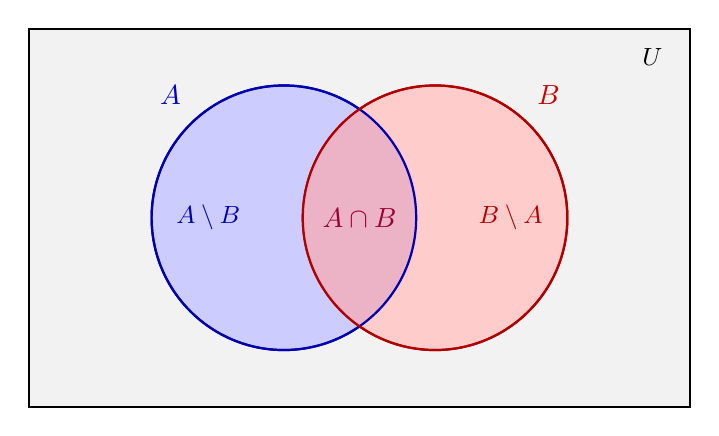
\begin{tikzpicture}[scale=1.2]

  % Universe box
  \fill[gray!10] (-3.5, -2) rectangle (3.5, 2);
  \draw[thick] (-3.5, -2) rectangle (3.5, 2);
  \node[font=\small] at (3.1, 1.7) {$U$};

  % A circle
  \fill[blue!20] (-0.8, 0) circle (1.4cm);
  \draw[thick, blue!70!black] (-0.8, 0) circle (1.4cm);

  % B circle
  \fill[red!20] (0.8, 0) circle (1.4cm);
  \draw[thick, red!70!black] (0.8, 0) circle (1.4cm);

  % Intersection fill
  \begin{scope}
    \clip (-0.8, 0) circle (1.4cm);
    \fill[purple!30] (0.8, 0) circle (1.4cm);
  \end{scope}

  % Redraw outlines on top
  \draw[thick, blue!70!black] (-0.8, 0) circle (1.4cm);
  \draw[thick, red!70!black] (0.8, 0) circle (1.4cm);

  % Labels
  \node[blue!80!black,   font=\bfseries] at (-2.0,  1.3) {$A$};
  \node[red!80!black,    font=\bfseries] at ( 2.0,  1.3) {$B$};
  \node[purple!80!black, font=\bfseries] at ( 0,    0  ) {$A \cap B$};

  % A only region
  \node[blue!70!black, font=\small] at (-1.6, 0) {$A \setminus B$};

  % B only region
  \node[red!70!black, font=\small] at (1.6, 0) {$B \setminus A$};

\end{tikzpicture}
\end{center}
Consider this diagram again, for both questions. We will first find, with proof, an explicit form of $(A \cup B)'$, then do the same for $(A \cap B)'$.
\begin{proof}
To simplify this, we will try to derive a form for the expression in terms of $A'$ and $B'$. First, let us consider a third set $C = U \setminus (A \cup B)$ (all the gray area). Now, the total set $U$ is broken up into four separate sets
\begin{enumerate}
\item $A \setminus B$ - the blue space
\item $B \setminus A$ - the red space
\item $A \cap B$ - the purple space
\item $C := U \setminus (A \cup B)$ - the gray space
\end{enumerate}

Note that $C$ is essentially the same as $(A \cup B)'$, since by definition, the complement is the set complement with the universal set $U$. We now want to construct $C$ a different way. 

First, consider the set 
\[
A' = (B \setminus A) \cup C
\]
Similarly, 
\[
B' = (A \setminus B) \cup C
\]
Then, since we are simply seeking an expression for $C$, we can use these compositions of $A'$ and $B'$ to construct one. We consider
\[
A' \cap B' = ((B \setminus A) \cup C) \cap ((A \setminus B) \cup C) = 
\]
\[
((B \setminus A) \cap (A \setminus B)) \cup ( (B \setminus A) \cap C) \cup (C \cap (A \setminus B)) \cup (C \cap C)
\]
First, note that by definition,
\[
(B \setminus A) \cap (A \setminus B) = \emptyset
\]
Furthermore, $(B \setminus A) \cap C = \emptyset$ and $(A \setminus B) \cap C = \emptyset$ by the definition of these sets.
\[
A' \cap B' = \emptyset\cup \emptyset\cup\emptyset\cup C = C
\]
Therefore
\[
(A \cup B)' = C = A' \cap B'
\]
We now turn our attention to finding $(A \cap B)'$. In a similar manner, consider 
\[
A' \cup B' = ((B \setminus A) \cup C) \cup ((A \setminus B) \cup C)
\]
\[
= B \setminus A \cup A \setminus B \cup C
\]
which is exactly the union of the blue, red, and gray areas. This union defines $(A \cap B)'$, which we know to also be the union of the blue, red, and gray areas. Therefore, 
\[
(A \cap B)' = B \setminus A \cup A \setminus B \cup C = A' \cup B'
\]
\end{proof}

This set of equations
\[
\begin{cases}
(A \cup B)' = A' \cap B' \\
(A \cap B)' = A' \cup B'
\end{cases}
\]
is known as De'Morgan's Laws. They are a useful and perhaps counterintuitive result in set theory (often extended to logic as well - you may have seen this in truth tables). 
\end{sol}

\begin{sol}{Problem 2.3}
We will follow a proof by mathematician Georg Cantor. This proof uses a concept of a bijection, which you may have not yet seen. While we have not discussed bijections in their full formality, we will use them loosely (you will understand the logic behind this). 
\begin{proof}
If $|\mathbb{Z}| = | \mathbb{N}|$, then we can construct a function $f: \mathbb{N} \to \mathbb{Z}$ such that each element of $\mathbb{N}$ maps to a single, unique element of $\mathbb{Z}$. This is known formally as an injective mapping or injective function. 
\[
x, y \in \mathbb{N}, f(x) = f(y) \iff x = y
\]
We also must prove that we can "access" all elements of $\mathbb{Z}$ via this mapping, that 
\[
\forall z \in \mathbb{Z}, \exists n \in \mathbb{N} \text{ such that } f(n) = z
\]
Therefore, the function $f$ has a "range" that spans the entire set of integers $\mathbb{Z}$. This is known more formally as a surjective map or surjective function. 

If a map or function is both injective and surjective, we call it bijective. Bijective maps are of special interest, because we can pair every element of the domain to a unique element in the range. In this case, if we find that there exists a bijective map $f:\mathbb{N} \to \mathbb{Z}$ (or $f^{-1}: \mathbb{Z} \to \mathbb{N}$), then every element of $\mathbb{N}$ corresponds to a unique element of $\mathbb{Z}$, and every element of $\mathbb{Z}$ corresponds to a unique element of $\mathbb{N}$. In this way, we pair every element of both sets, exhaustively. A simple bijective map between the natural numbers and integers would be
\[
f(0) = 0
\]
\[
 f(1) = 1
\]
\[
f(2) = -1
\]
\[
f(3) = 2
\]
\[
f(4) = -2
\]
\[
f(5) = 3
\]
and so on. We can write this more formally as 
\[
f(n) = 
\begin{cases}
-\frac{n}{2} ~~ \text{if $2 \mid n$}\\
\frac{n+1}{2} ~~ \text{if $ 2 \nmid n$}
\end{cases}
\]
we can see that first, each natural number $n$ will output one unique integer such that no other number will output the same integer. Therefore, $f$ is injective. Second, we will eventually list every single integer this way, so this is also surjective. Since $f$ is a bijective function between natural numbers and the integers, we know that we can pair every single natrual number with every single integer. Therefore
\[
|\mathbb{N}| = |\mathbb{Z}|
\]
\end{proof}

While this was not the most formal introduction to injectiveity, surjectivity, and bijectivity, it should help you show that if there exists a bijective map between two sets, then they are of the same cardinality. Bijective maps/functions are also very important across many spaces, from competition math to linear algebra. As a fun fact, a function only has a well-defined inverse if it is a bijective function. There are many more properties of bijective functions; this is just the tip of the iceberg. You can already begin to see how useful this concept is!

This is a surprising result that concerned many mathematicians, and may concern you if seen for the first time. It seems that obviously there are more integers than natural numbers, since we are including negatives in one but not the other. However, the properties of infinite sets are weird!
\end{sol}


\begin{sol}{Problem 2.4}
\begin{center}
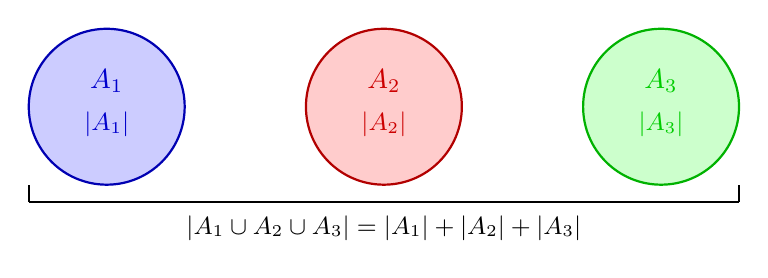
\begin{tikzpicture}[scale=1.1]

  % Three disjoint circles
  \fill[blue!20]  (-3.2, 0) circle (0.9cm);
  \fill[red!20]   ( 0,   0) circle (0.9cm);
  \fill[green!20] ( 3.2, 0) circle (0.9cm);

  \draw[thick, blue!70!black]  (-3.2, 0) circle (0.9cm);
  \draw[thick, red!70!black]   ( 0,   0) circle (0.9cm);
  \draw[thick, green!70!black] ( 3.2, 0) circle (0.9cm);

  \node[blue!80!black,  font=\bfseries] at (-3.2,  0.3) {$A_1$};
  \node[red!80!black,   font=\bfseries] at ( 0,    0.3) {$A_2$};
  \node[green!80!black, font=\bfseries] at ( 3.2,  0.3) {$A_3$};

  \node[blue!80!black,  font=\small] at (-3.2, -0.2) {$|A_1|$};
  \node[red!80!black,   font=\small] at ( 0,   -0.2) {$|A_2|$};
  \node[green!80!black, font=\small] at ( 3.2, -0.2) {$|A_3|$};

  % Union diagram belo

    % Brace underneath
    \draw[thick] (-4.1, -1.1) -- (4.1, -1.1);
    \draw[thick] (-4.1, -1.1) -- (-4.1, -0.9);
    \draw[thick] ( 4.1, -1.1) -- ( 4.1, -0.9);

    \node[font=\small] at (0, -1.4) 
      {$|A_1 \cup A_2 \cup A_3| = |A_1| + |A_2| + |A_3|$};

\end{tikzpicture}
\end{center}
When sets are pairwise mutually exclusive, they share no elements - the circles do not overlap. Counting the union is therefore the same as counting each set separately and adding, since no element is counted twice.
\end{sol}

\begin{sol}{Problem 2.5}
The negation is: "$n^2$ is a multiple of 3 and $n$ is not a multiple of 3". 

The contrapositive is: "if $n$ is not a multiple of 3, then $n^2$ is not a multiple of 3".

the converse is: "if $n$ is a multiple of 3, then $n^2$ is a multiple of 3".
\end{sol}

\begin{sol}{Problem 2.6}
We first consider how an element of the power set is constructed. Every subset of $A$ is formed by making a binary choice for each element of $A$: either we include it or we exclude it. Since these choices are independent across all $n$ elements, the total number of distinct subsets is $2^n$. More formally,

\begin{proof}
Let $A$ be a finite set with $|A| = n$. For each element $a_i \in A$ where $1 \leq i \leq n$, define an indicator variable $x_i \in \{0, 1\}$, where $x_i = 1$ denotes inclusion of $a_i$ in a subset and $x_i = 0$ denotes exclusion. Every subset of $A$ corresponds uniquely to a tuple $(x_1, x_2, \ldots, x_n) \in \{0,1\}^n$, and every such tuple corresponds uniquely to a subset of $A$. This is a bijection between $\mathcal{P}(A)$ and $\{0,1\}^n$. Therefore,
\[
|\mathcal{P}(A)| = |\{0,1\}^n| = \underbrace{2 \times 2 \times \cdots \times 2}_{n \text{ times}} = 2^n
\]
\end{proof}
For example, if $A = \{1, 2, 3\}$, the tuple $(1, 0, 1)$ corresponds to the 
subset $\{1, 3\}$, and $(0, 0, 0)$ corresponds to $\emptyset$. All $2^3 = 8$ 
tuples account for all $8$ subsets of $A$.

As an aside, this result has a important connection to infinite sets. It can be shown that $|\mathcal{P}(\mathbb{N})| = |\mathbb{R}|$. This is why $|\mathbb{R}| = 2^{\aleph_0}$. In other words, the uncountable infinity of the real numbers is precisely the infinity of all possible subsets of the natural numbers, a perhaps unexpected connection between these concepts.
\end{sol}

\begin{sol}{Problem 2.7}
It is valid (though not standard) that sets contain themselves. For example, we can define a set 
\[
A = \{ A, \{ 1\}\}
\]
which is a perfectly valid set (though this makes people uncomfortable). 

The set of all sets that contain themselves is a little more abstract. However, it does exist. This set would again contain itself, but is still a valid set (though it is scary to think about). We know, just as a fun fact, that this set of all sets that contain themselves would contain both the set $A$, and itself. Though it is much harder to characterize. 

The final question is a lot harder. Consider that the set of all sets that does not contain themselves exist. Call this set $\Omega$. Does $\Omega$ contain itself? If $\Omega$ did contain itself, that means that $\Omega$ would not be the set of all sets that contain themselves since $\Omega$ includes itself, which in turn includes itself, and so on. Therefore, there exists a set in $\Omega$ that contains itself. This is a contradiction. Now, say that $\Omega$ did not contain itself. This immediately contradicts the definition of $\Omega$. If $\Omega$ does not contain itself, then $\Omega$ should be in the set $\Omega$, which is by definition the set of all sets that don't contain themselves. Confusing! Try to reason through the explanation multiple times, drawing pictures if needed. This is a difficult concepts, and seems to set on fire the convention of sets! 

If it may help you, I liken this paradox (known as Russell's Paradox) to something I call Pinocchio's Paradox. Assume Pinocchio's nose grows every time he lies, and shrinks every time he tells the truth. What happens if he says "I am lying"? The best answer seems that the universe will just come to an end!; our system of logic cannot handle situations like these. Similarly, our system of sets breaks down when we consider the set of all sets that do not contain themselves. Russell's paradox has challenged the definition of sets: simply saying a set is a collection of things is not enough. This has led to the rise of more formal rules about sets, developed by Zermelo and Franekel and appropriately named Zermelo-Fraenkel set theory (ZF or ZFC). 
\end{sol}